\chapter{Market Analysis and Related Work}
\label{ch:ma}

\section{Introduction}
This chapter situates the Echora project within the broader context of assistive technologies for Blind and Low Vision (BLV) users. It examines the current market landscape, existing solutions, and relevant research efforts to identify gaps, limitations, and opportunities that motivate the proposed system.

The market analysis explores commercial and emerging assistive products, evaluating their strengths, weaknesses, and positioning through structured analytical frameworks. This analysis provides insight into user needs, technological trends, and external factors influencing the development and adoption of assistive systems.

In addition, this chapter reviews relevant academic literature and related systems that address sensory substitution, navigation assistance, and object interaction. By analyzing prior work and existing approaches, the chapter highlights how Echora differs from and builds upon current solutions.

Together, the market analysis, literature review, and related work establish a comprehensive foundation for understanding the need for Echora and justify its design choices. The findings of this chapter inform the system design and implementation presented in subsequent chapters.


\section{Market Analysis}

The market analysis for Echora examines the current landscape of assistive technologies designed for Blind and Low Vision (BLV) users, with particular emphasis on navigation, object interaction, and sensory substitution systems. Existing solutions range from OCR-based smart glasses and wearable obstacle detectors to smartphone-assisted navigation aids. While these systems address specific user needs, they often focus on a single modality or task, such as text reading or basic obstacle detection.

This analysis evaluates the strengths, limitations, and positioning of current solutions to identify gaps in functionality, usability, and integration. By applying structured analytical frameworks, including SWOT, the 7P’s marketing mix, and PESTEL analysis, the section highlights both internal and external factors influencing product adoption and technological feasibility.

The insights gained from this analysis inform the design decisions of Echora and clarify how the proposed system differentiates itself through sensor fusion, multimodal feedback, and support for both macro-navigation and micro-interaction. The following subsections present these analyses and visual comparisons in detail.

\newpage
\subsection{SWOT Analysis}
\begin{figure}[H]
\raggedright
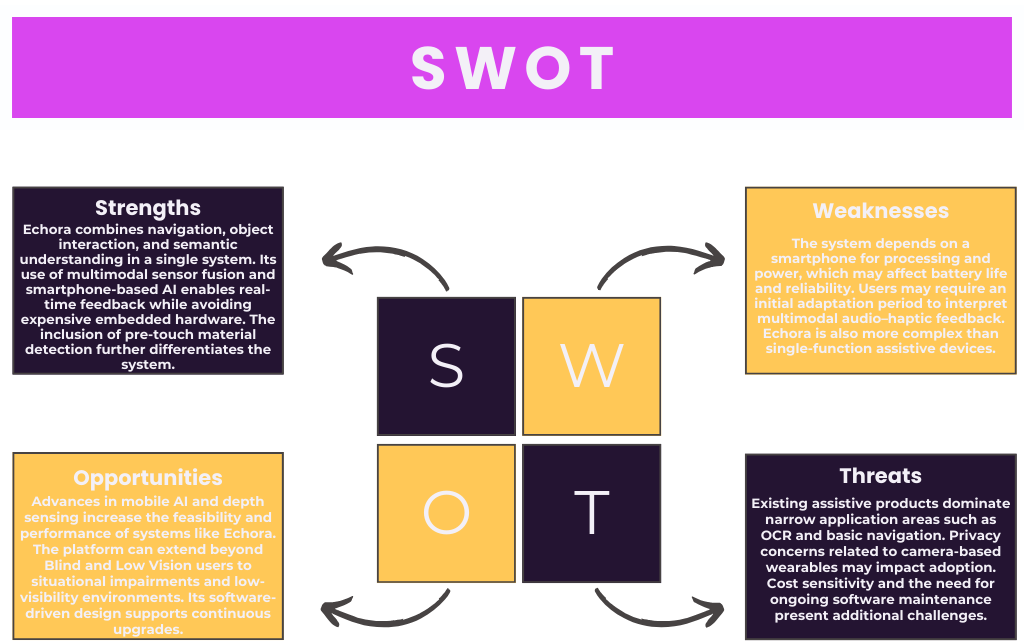
\includegraphics[height=0.7\textwidth]{assets/SWOT.png}
\caption{SWOT Analysis Diagram}
\label{fig:swot}
\end{figure}

\newpage
\subsection{7 P’s}
\begin{figure}[H]
\raggedright
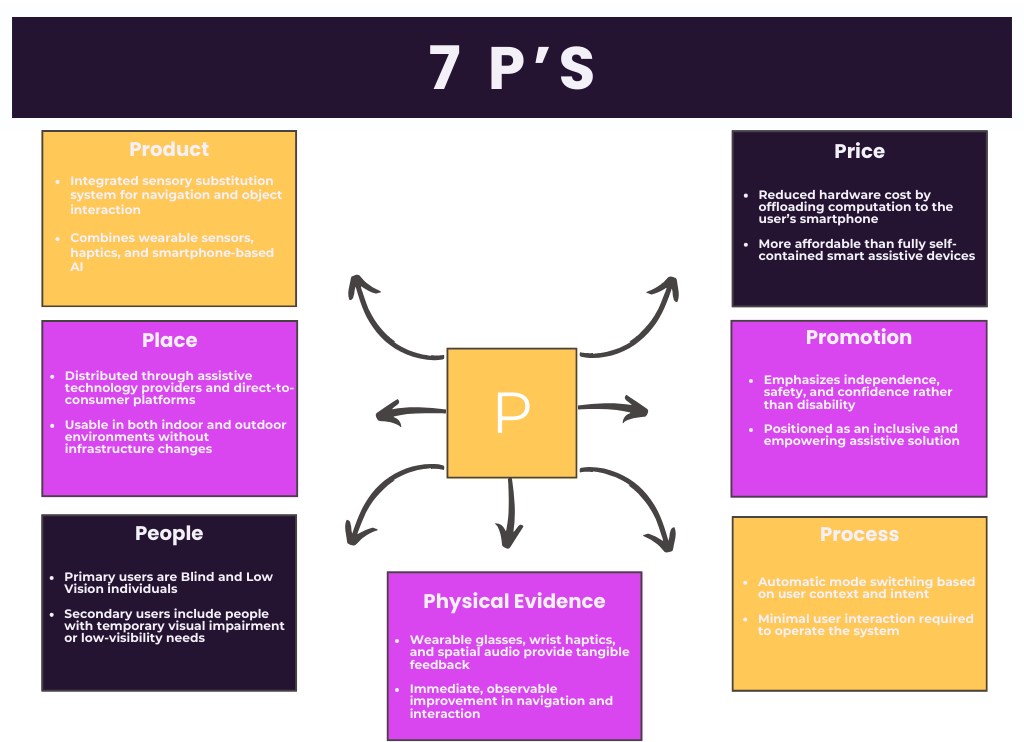
\includegraphics[height=0.8\textwidth]{assets/7 P's.png}
\caption{7P's Diagram}
\label{fig:seven_ps}
\end{figure}

\newpage
\subsection{PESTEL Analysis}
\begin{figure}[H]
\raggedright
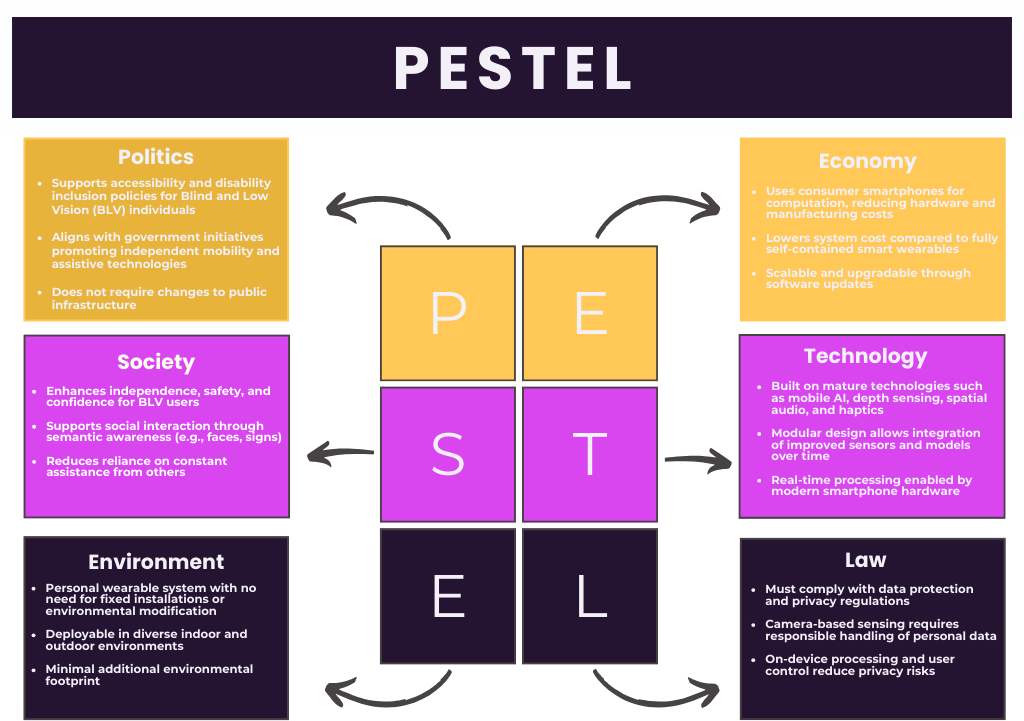
\includegraphics[height=0.8\textwidth]{assets/PESTEL.png}
\caption{PESTEL Analysis Diagram}
\label{fig:pestel}
\end{figure}

\newpage
\subsection{Similar Projects}

\subsubsection{Envision Glasses}
\begin{figure}[H]
\raggedright
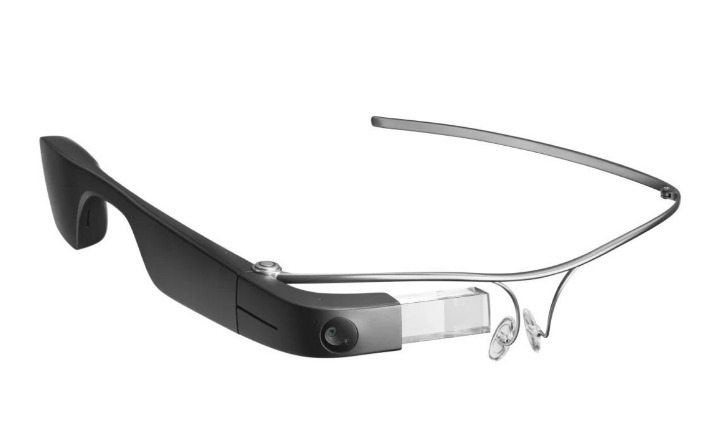
\includegraphics[width=0.5\textwidth]{assets/Envision Glasses.jpg}
\caption{Envision Glasses}
\label{fig:envision}
\end{figure}

\begin{tcolorbox}[breakable,colback=blue!4,colframe=blue!35,title=\textbf{Envision Glasses Summary}]
\textbf{Description:} Envision Glasses are smart glasses designed primarily for text recognition and scene description. The system relies on a camera and smartphone-based AI to provide audio feedback about visible text and objects.

\medskip
The key features of the system include optical character recognition (OCR), object and scene description, and face recognition. The main advantages of Envision Glasses include strong text-reading performance, a well-established commercial product ecosystem, and ease of use for reading and identification tasks. However, the system does not provide 3D spatial navigation support and does not include haptic feedback. It also does not offer hand guidance or object interaction support, and it lacks depth sensing, which limits its ability to provide continuous spatial awareness.
\end{tcolorbox}


\subsubsection{Seleste Glasses}
\begin{figure}[H]
\raggedright
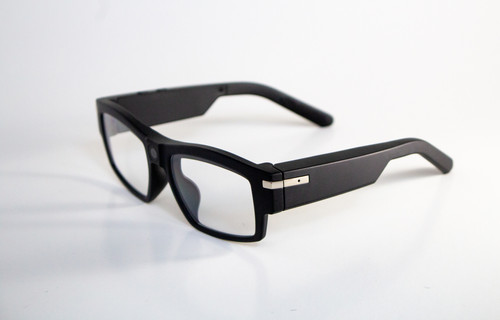
\includegraphics[width=0.5\textwidth]{assets/Seleste Glasses.jpg}
\caption{Seleste Glasses}
\label{fig:seleste}
\end{figure}

\begin{tcolorbox}[breakable,colback=blue!4,colframe=blue!35,title=\textbf{Seleste Glasses Summary}]
\textbf{Description:} Seleste Glasses are lightweight smart glasses that depend heavily on smartphone vision processing. The system focuses on visual interpretation but offers limited spatial understanding.

\medskip
The system provides camera-based scene interpretation supported by smartphone AI processing. Its advantages include lightweight hardware design and the flexibility of leveraging smartphone compute. Nevertheless, the system does not provide 3D navigation or depth awareness and does not include haptic feedback. It also lacks object interaction features and hand guidance, resulting in limited assistive functionality when compared to integrated perception systems.
\end{tcolorbox}


\subsubsection{OrCam MyEye}
\begin{figure}[H]
\raggedright
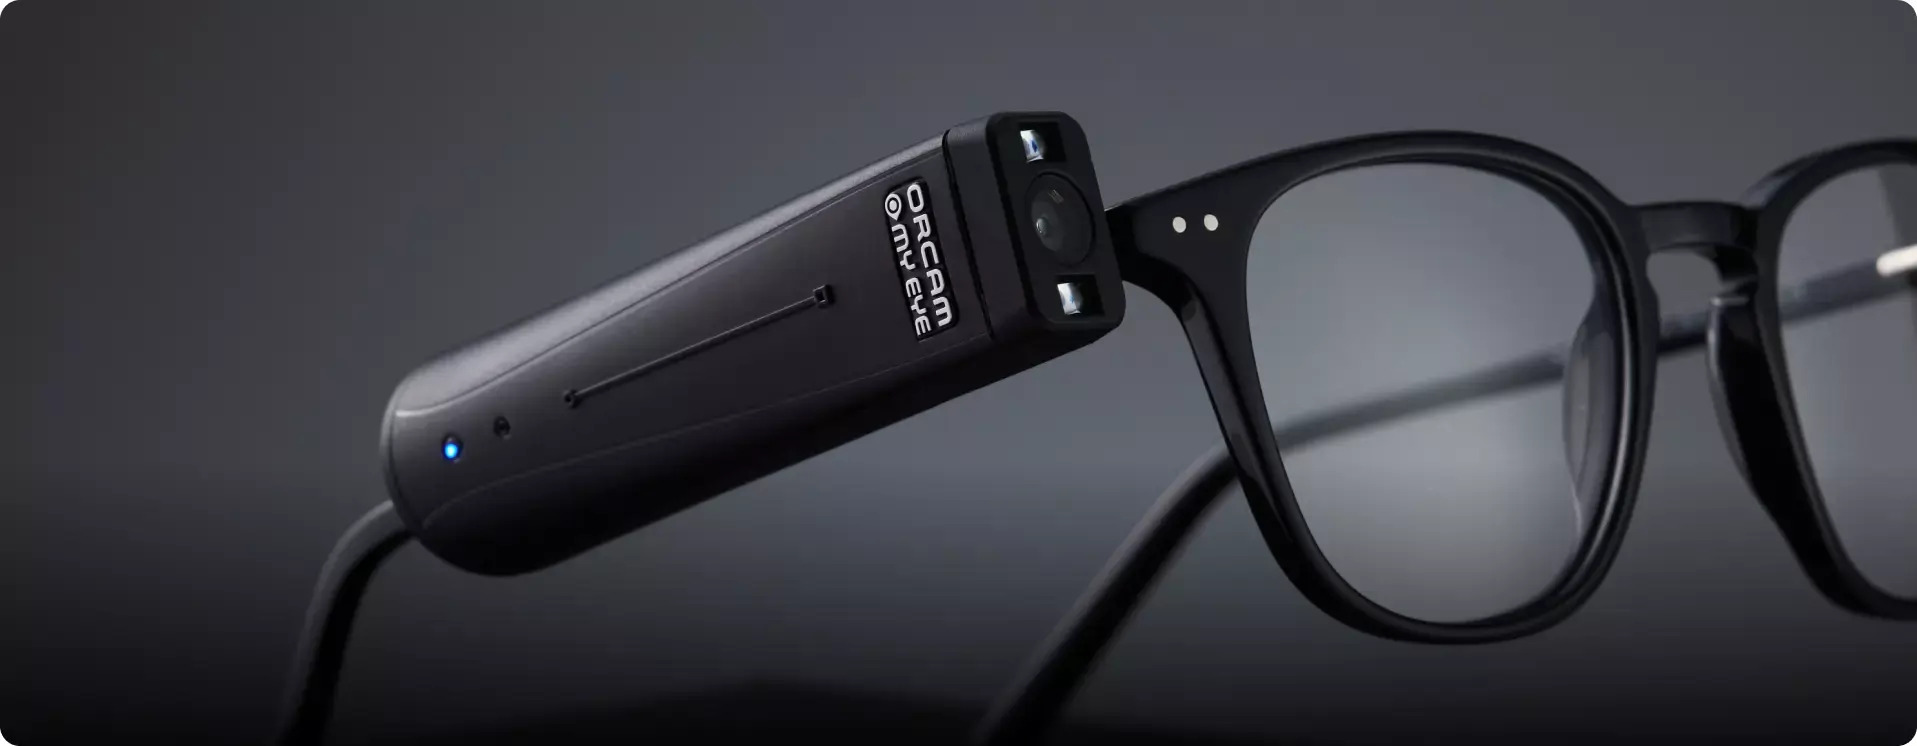
\includegraphics[width=0.85\textwidth]{assets/OrCam MyEye.jpg}
\caption{OrCam MyEye}
\label{fig:orcam}
\end{figure}

\begin{tcolorbox}[breakable,colback=blue!4,colframe=blue!35,title=\textbf{OrCam MyEye Summary}]
\textbf{Description:} OrCam MyEye is a wearable camera that clips onto glasses and provides audio feedback for text reading and face recognition. It is designed for quick access to visual information rather than spatial awareness.

\medskip
The key functions include OCR for printed and digital text, face recognition, and object identification. The system achieves high-quality OCR performance and is designed to be compact, lightweight, and usable with minimal interaction. However, it does not support navigation or obstacle avoidance, and it does not provide depth perception. Additionally, it does not include haptic feedback or interaction support, and its assistance is largely limited to semantic outputs rather than continuous spatial understanding.
\end{tcolorbox}


\subsubsection{WeWalk Smart Cane}
\begin{figure}[H]
\raggedright
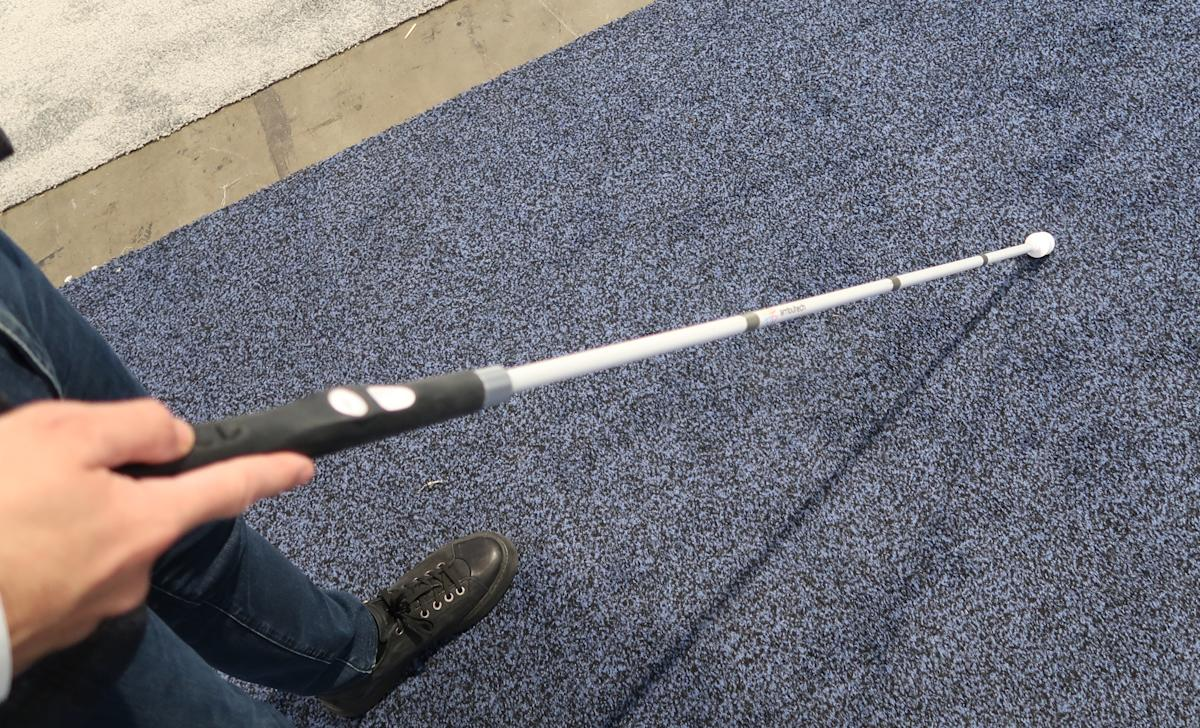
\includegraphics[width=0.5\textwidth]{assets/WeWalk Smart Cane.jpeg}
\caption{WeWalk Smart Cane}
\label{fig:wewalk}
\end{figure}

\begin{tcolorbox}[breakable,colback=blue!4,colframe=blue!35,title=\textbf{WeWalk Smart Cane Summary}]
\textbf{Description:} WeWalk is a smart cane that enhances traditional white cane use with ultrasonic sensors and vibration feedback to detect nearby obstacles.

\medskip
The system supports ultrasonic obstacle detection, vibrotactile feedback, and smartphone connectivity for extended functionality. Its main strengths include a familiar form factor for BLV users, simple and intuitive obstacle alerts, and strong compatibility with conventional cane usage. However, its sensing is limited to basic forward obstacle detection and it does not provide semantic understanding of objects. It also does not support hand guidance or object interaction tasks, and it does not construct a 3D environmental map.
\end{tcolorbox}


\subsubsection{Sunu Band}
\begin{figure}[H]
\raggedright
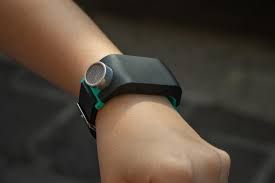
\includegraphics[width=0.5\textwidth]{assets/Sunu Band.jpeg}
\caption{Sunu Band}
\label{fig:sunu}
\end{figure}

\begin{tcolorbox}[breakable,colback=blue!4,colframe=blue!35,title=\textbf{Sunu Band Summary}]
\textbf{Description:} Sunu Band is a wrist-worn ultrasonic device that alerts users to nearby obstacles using vibration patterns. It is designed for basic spatial awareness rather than detailed perception.

\medskip
The device provides ultrasonic proximity sensing and vibrotactile alerts in a compact wrist-worn design. Its advantages include portability, low wearability burden, and a simple feedback mechanism that is useful for short-range obstacle detection. Despite these strengths, the device does not provide object recognition or classification and does not perform depth mapping or navigation planning. It also does not support hand guidance or semantic feedback, resulting in limited environmental understanding.
\end{tcolorbox}

\newpage
\begin{table}[H]
\raggedright
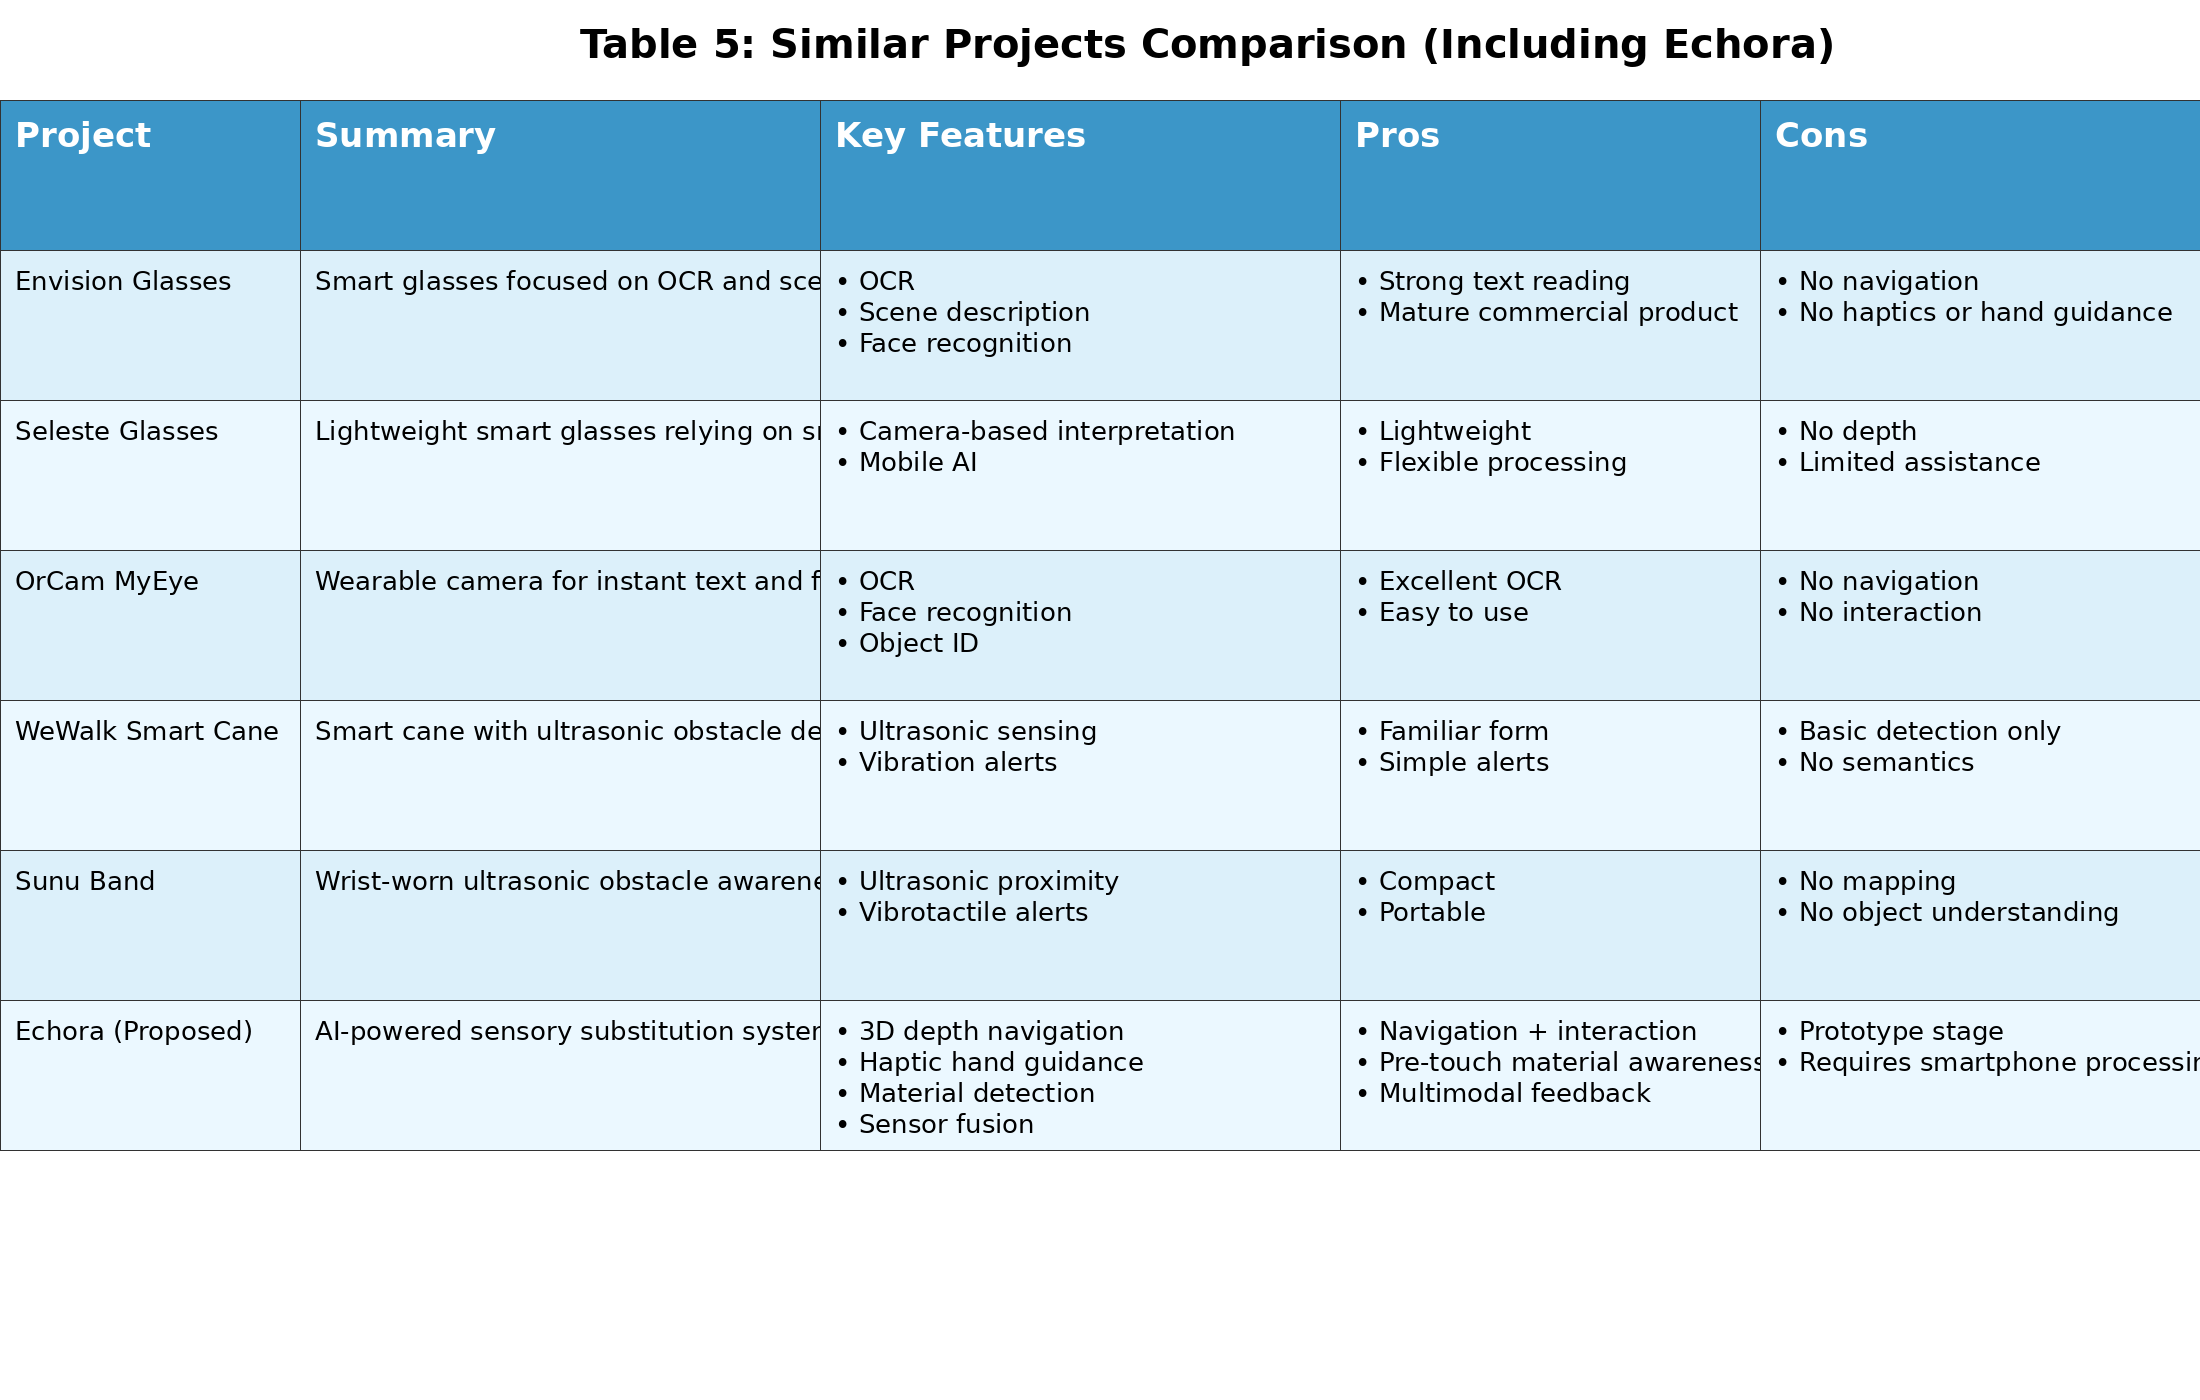
\includegraphics[height=0.7\textwidth]{assets/similar_projects_comparison_echora.png}
\caption{Comparison of Existing Assistive Technologies and the Proposed Echora System}
\label{tab:comparison}
\end{table}


\section{Literature Review}
\label{sec:literature_review}

This section reviews prior work that informs Echora’s design, focusing on spatial-audio navigation, learnable visual-to-audio mappings, robust 3D world modeling, haptic wearables for guidance, and hand-centered interaction systems. Together, these works motivate Echora’s sensor-fusion approach and the separation between macro-navigation and micro-interaction.

\subsubsection{Spatial Audio for Navigation and Obstacle Avoidance}
\label{subsec:lit_spatial_audio}

A core direction in assistive navigation is converting spatial structure into 3D audio cues that represent obstacle proximity and layout. EchoSee introduces a mobile navigation approach that aligns closely with Echora’s macro-navigation goal by using an iPhone LiDAR scanner to build a live 3D map and applying raycasting to place virtual audio sources on surrounding surfaces, producing a spatial-audio soundscape. In feasibility testing, EchoSee reported a substantial reduction in obstacle collisions of approximately 40\%, indicating that continuous spatial sonification can support safer mobility without relying only on spoken alerts \cite{echosee}. This supports Echora’s approach of building a continuous sound-world rather than using discrete warning messages alone.

\subsubsection{Visual-to-Auditory Sensory Substitution as a Learnable Mapping}
\label{subsec:lit_visual_to_audio}

Another established strategy maps visual depth and geometry to simple audio parameters that users can learn quickly. Easy-Access SoundView converts a small set of visual points into audio cues where vertical position maps to pitch and depth maps to volume. The study reports that the mapping is easy to learn and that blind participants could navigate obstacle courses from early trials, validating that minimal and intuitive audio encodings can be effective when carefully designed \cite{soundview}. For Echora, this work provides a practical baseline mapping strategy for early prototyping before moving to richer 3D generative audio scenes.

\subsubsection{Robust Environment Mapping as the Foundation for Assistive World Models}
\label{subsec:lit_world_models}

Reliable macro-navigation requires a stable spatial model of the environment. RGB-D mapping approaches build dense 3D indoor maps using depth alignment together with visual feature tracking to maintain accuracy even in challenging conditions such as low-texture surfaces or poor lighting. This directly supports Echora’s use of depth and vision fusion to improve map stability, which in turn affects the quality of audio placement and collision warnings in a sound-world navigation system \cite{rgbd_mapping}.

\subsubsection{Haptic Wearables for Sensory Replacement and Guidance}
\label{subsec:lit_haptics}

Haptic feedback is widely used to reduce cognitive load from audio and to provide directional or proximity cues through the body. A broad review of haptic wearables categorizes systems into sensory replacement, sensory augmentation, and training devices, and surveys multiple applications including navigation and obstacle avoidance. These findings support Echora’s wrist-based haptic approach, in which a wrist-mounted haptic actuator is used to deliver directional and proximity feedback for navigation, collision avoidance, and fine-grained task-level guidance \cite{shull_damian2015}.

\subsubsection{Hands-Based Tactile Perception for Object Interaction (Micro-Interaction)}
\label{subsec:lit_hands}

While many assistive systems focus primarily on navigation, Seeing With the Hands (CHI~’25) shifts sensory substitution toward manual interaction, arguing that the hand’s perspective is ergonomic and flexible for object exploration. The authors prototype a wrist-mounted camera and render tactile images through an electrotactile array on the back of the hand, enabling Blind and Low Vision users to complete object-related tasks. Importantly, participants preferred combining both eye-view and hand-view perspectives, using one for overview and the other for detail. This directly motivates Echora’s separation of macro-navigation and micro-interaction feedback, and supports multimodal fusion rather than replacing one modality entirely \cite{seeing_with_the_hands_chi25}.

\subsubsection{Smart Glasses Prototypes for OCR-Based Assistance and Practical Constraints}
\label{subsec:lit_ocr_glasses}

OCR-centered smart-glasses prototypes demonstrate the value of text access but also reveal practical constraints relevant to Echora. A smart-glasses system using text detection and OCR reports strong text recognition performance, but also highlights real-world limitations such as language support constraints, effective capture distance, and ergonomic considerations for mounting and comfort. For Echora, these findings emphasize the importance of wearable comfort, robust sensing under varied conditions, and fallback strategies when camera-based perception is unreliable \cite{smart_glasses_for_blind_people}.

\subsubsection{Deep Learning Wearables for Navigation (Vision + Sensors)}
\label{subsec:lit_dl_wearables}

Recent wearable navigation systems show that real-time deep learning can be feasible when models are lightweight and when sensors are combined. A low-cost wearable and smart-cane hybrid integrates vision-based perception with ultrasonic sensing and GPS augmentation, and reports comparative results indicating that modern object-detection approaches can achieve practical accuracy and frame rates. For Echora, this reinforces the feasibility of on-device real-time inference and supports the project’s emphasis on sensor fusion to improve robustness and safety compared to relying on a single sensing modality \cite{kumar_jain_2022}.

\newpage
\begin{table}[H]
\raggedright
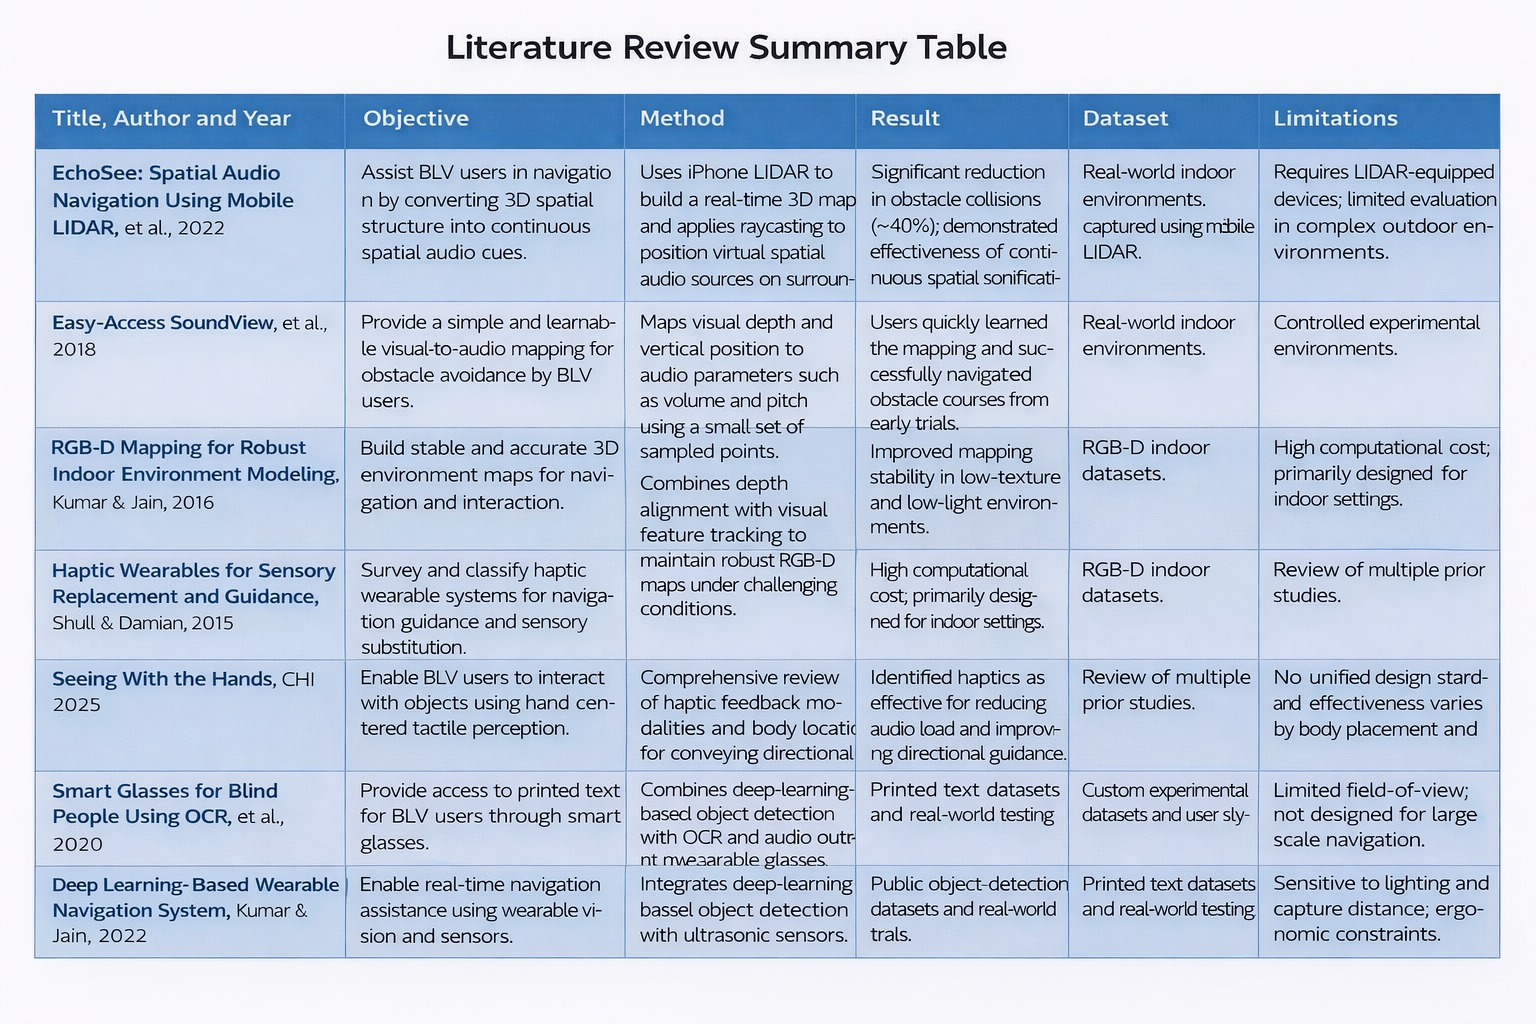
\includegraphics[height=0.73\textwidth]{assets/Literature Review.png}
\caption{Literature Review Summary Table}
\label{tab:lit_review_table}
\end{table}

\section{Background}

The integration of artificial intelligence (AI), machine learning (ML), and wearable sensing technologies has significantly advanced assistive systems for Blind and Low Vision (BLV) individuals. Modern assistive devices increasingly rely on computer vision, depth sensing, haptics, and audio feedback to compensate for the loss of visual perception. These technologies aim to provide users with spatial awareness, object recognition, and navigation support in real time, enabling safer and more independent interaction with their environment. However, designing systems that are both computationally efficient and perceptually intuitive remains a key challenge, particularly in wearable and mobile contexts.

Sensory substitution systems translate visual information into alternative sensory modalities such as sound or touch. Early sensory substitution approaches demonstrated that spatial layouts and object features could be conveyed through auditory or tactile feedback. Recent advances have expanded these systems using depth cameras, spatial audio, and haptic interfaces to improve environmental understanding. Despite their effectiveness in navigation tasks, many sensory substitution systems focus primarily on global spatial awareness and provide limited support for fine-grained object interaction.

Computer vision and depth sensing play a central role in modern assistive technologies. Depth cameras and RGB-D sensors enable the reconstruction of three-dimensional representations of the environment, supporting obstacle detection, distance estimation, and spatial mapping. These techniques allow systems to perceive structural elements such as walls, doors, and furniture. However, processing depth data in real time requires efficient algorithms and hardware acceleration, especially when deployed on mobile devices with limited computational resources.

Machine learning models, particularly Convolutional Neural Networks (CNNs), are widely used for visual perception tasks such as object detection, text recognition, and scene understanding. CNNs excel at extracting spatial features from images and depth maps, making them suitable for assistive applications that require real-time perception. While these models provide high accuracy, their computational demands pose challenges for wearable systems, motivating the use of smartphone-based processing rather than fully embedded solutions.

Haptic feedback and hand guidance have been explored as effective methods for conveying spatial and directional information non-visually. Vibrotactile and electrotactile interfaces can guide user motion by encoding direction, distance, and urgency through tactile patterns. Hand-centered haptic guidance has been shown to support precise object interaction by providing feedback relative to the user’s hand position. However, most existing systems rely on predefined targets or simple proximity cues, limiting their flexibility in unstructured environments.

Multimodal sensor fusion combines data from vision, depth, inertial sensors, and active acoustics to provide a more robust and comprehensive perception of the environment. By integrating multiple sensory inputs, assistive systems can adapt feedback based on user context and intent. Nevertheless, achieving low-latency fusion and intuitive feedback remains challenging, particularly in real-time mobile applications.

In summary, prior research highlights significant progress in sensory substitution, computer vision, haptics, and machine learning for assistive technologies. However, challenges related to real-time performance, fine-grained interaction, and pre-contact object understanding persist. These limitations motivate the design of integrated systems, such as Echora, that unify navigation, interaction, and semantic understanding through a single adaptive framework.


\section{Summary}

This chapter examined the market landscape, existing assistive technologies, and relevant research related to sensory substitution systems for Blind and Low Vision users. The market analysis showed that current commercial solutions are largely fragmented, with most devices addressing isolated tasks such as text recognition or basic obstacle detection. SWOT, PESTEL, and marketing analyses highlighted both the opportunities enabled by advances in mobile AI and wearable sensing, as well as the limitations and challenges faced by existing systems.

The literature review and related work demonstrated that sensory substitution, depth-based perception, haptic guidance, and mobile-based AI are viable approaches for supporting navigation and interaction. However, prior systems typically focus on either environmental awareness or object-level interaction, rarely combining both within a single adaptive framework.

These findings motivate the design of Echora as an integrated sensory substitution system that unifies navigation, hand-level interaction, and semantic understanding through real-time multimodal sensor fusion. The next chapter presents the system design and architecture of Echora, detailing how these concepts are realized in practice.
